\subsection{Hysteresis Switch}

Hysteresis can be used to filter signals so that the output reacts
slowly by taking recent history into account.  For example, a
controller may turn on a pump when the water level drops below level
A, but not turn it off until the water level rises above level B.
This controller has hysteresis.  Thus the on/off output of controller
to the pump when the water level is between A and B depends on the
history of the water level.  This prevents rapid switching on and off
as the water levels drift around the set point.

The Hysteresis Switch assessor approximates the behavior of a
hysteresis controller, where a water level monitor is used as a signal
with specified on and off water levels.  The relative position of the
ON and OFF levels (Figure \ref{fig:HysteresisSwitch}) determines if
the pump is turned on when water levels drop below the ON level (``OFF
on top'') or when water levels rise above the ON level (``ON on
top'').

\begin{figure}[!htb]
 \begin{center}
  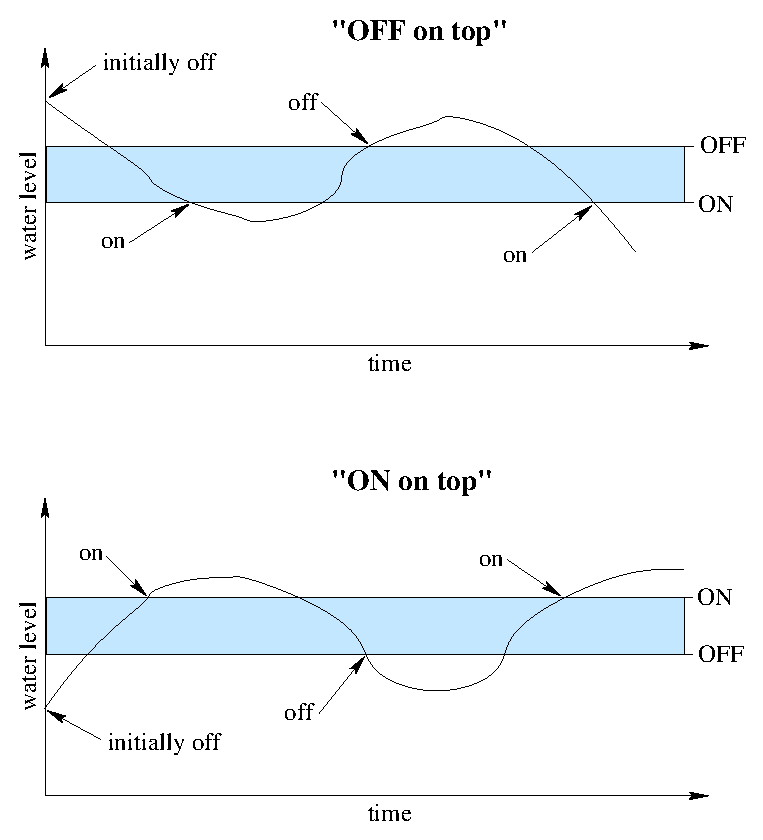
\includegraphics[scale=.5]{Graphics/hysteresis}
  \caption{\label{fig:HysteresisSwitch} Relative position of ON and OFF levels for the {\tt HysteresisSwitch} assessor.}
 \end{center}
\end{figure}

The Hysteresis Switch is typically used by a regional manager
to control the operation of a pump.  The output from the Hysteresis
Switch assessor is 0.0 (off) or 1.0 (on) and can be monitored using an
assessor monitor with the attribute set to ``flow''.
